{\color{red}
\chapter[Amenity]{Incorporating amenity}\label{chapter-amenity}
% from Ricardo_Rent_and_Roemer_3.tex
% We will also include an urban wage premium. Otherwise the amenity factor is the only attractor. The wage premium provides a reason to travel to the city centre. The literature supports the notion that there is an  urban wage premium.  We will consider later how the premium arises from agglomeration externalities in production. 

%For workers, higher wages make them better off whereas higher rents make them worse off. Thus, greater consumption amenities in a city will make workers willing to accept both lower wages and higher rents. For firms, both higher wages and higher rents mean increased costs. Thus, localized productive advantages will make firms willing to accept higher wages and higher rents  \cite{pugaMagnitudeCausesAgglomeration2010}.
%.  This helps disentangle the consumption amenities from the productive advantages of big cities.

STILL WRITING. JUST READ THIS CHAPTER QUICKLY.

NEED AN INTRODUCTION TO EXPLAIN WHAT WE'RE TALKING ABOUT AND WHY, AND SCOPE OF THE CHAPTER.

We set the level of amenities to zero initially so we can focus on the productivity effects.  \glspl{amenity}, or non monetary income it another form of wealth, and it is %, are however, 
an important feature of the urban system. See Kaufmann et al. \cite{kaufmannScalingUrbanAmenities2022}. 
% We have intentionally suppressed amenity but can add it it simply.
% (ownership effects, produtivity spilllovers, - table where you show them in the static and dynamci case with amentity)
% 2 classes of exploratin of the model in the past tho chaptered
The previous two chapters on productivity \ref{chapter-ownership}, and productivity spillovers \ref{chapter-productivity-spillovers}, tested two hypotheses: first that financializaiton will change the ownership structure and second that there may be feedbacks from financiazation that actually reduce productivity in cities. This chapter introduces an extension of the model to study include \gls{amenity} and examines the effect of amenity on results.

CUT THIS PARAGRAPH? Basic New Economic Geography models posit two centripetal forces: economies of scale in manufacturing (\cite{gurwitzCatastrophicAgglomeration2019}) and households' preference for variety in the consumer goods they can buy; and \footnote{In NEG models the variety of consumption goods comes from increasing the number of  production sectors. Larger markets support more variety.} The agglomeration effects described in Chapters \ref{chapter-growth}, on growth,  running between local productivity  of exporting firms to population and then back to firm productivity provide the first of these centripetal forces leading to agglomeration. The second is an effect of growing complexity. 

CUT THIS PARAGRAPH? REPEATS STUFF WE'VE COVERED? Jane Jacobs was the first to define cities as problems of organized complexity. For Jacobs, a city is a system with many interrelated activities and markets in constant simultaneous change. Economic complexity gives rise to a class of consumption amenities that the New Economic Geography models exploit MODELS EXPLOIT?. In addition, the agglomeration of firms and people supports the growth of businesses that serve the local population. There is third general class of agglomeration effects however that  create a variety of amenities: the set of non-market intellectual and social benefits that come from access to other people, as well as the socially created services like libraries and communal activities.  

To understand amenity in our model, we need to understand it's relationship with growth, productivity, and agglomeration. Most of the literature on amenities deals with livability and the benefits for the individual. There is a strand in the literature, however, that links amenities to  growth. In 1954, for example, Edward Ullman \cite{ullmanAmenitiesFactorRegional1954} published  ``Amenities as a Factor in Regional Growth,'' an article that came to be seen in the geographical literature over the following 50 years as prescient \cite{walcottCommentsEdwardUllman2010} for introducing  the notion that amenities could be an important mobility magnet. 

Many have since extended this approach. Richard Florida, in a series of articles and books beginning in 2002 (see \cite{floridaCreativeClassEconomic2014}) examined the notion that urban growth depended on attracting  the creative class and that in turn rested in part on the amenities a city offered. A 2008  Statistics Canada study, `Cities and Growth: The Left Brain of North American Cities,' Beckstead et al  \cite{becksteadCitiesGrowthLeft2008} found substantial differences in average growth for cities with higher cultural employment and urban amenities.\footnote{Beckstead et al identify amenities with the unexplained median urban house price after controlling for median household income:  The basic premise would be that after conditioning on household income, variation in home prices across cities would be a function of the relative attractiveness of these places. The residuals  yield a continuous ranking of cities based on the estimated variation in urban amenities.} 
In 2023 Clark et al \cite{clarkAmenitiesDriveUrban2002} argue that much of Chicago's recent growth  should be attributed to reforms instituted by Mayor Richard M.  Daley  explicitly linked to amenities and quality of life issues, including parks and schools.

Boualam \cite{boualamDoesCultureAffect2014} provides evidence specialization in cultural occupations is not strong enough to affect factor prices at the city level, however. Abouy \cite{albouyWhatAreCities2016} finds that wage and housing cost differences across metropolitan areas are accounted for more by productivity than quality-of-life differences. Rappaport \cite{rappaportConsumptionAmenitiesCity2008}, on the other hand, presents empirical evidence  that amenities do support high-density levels, and that amenities  cause approximately one-fifth of the cross-sectional variation in metro population density. 

When positive urban amenities prevail, rents and housing prices will be higher in larger cities, but wages may be unaffected \cite{robackWagesRentsAmenities1988, dalmazzoAmenitiesSkillbiasedAgglomeration2011}. Dalmazzo and  de Blasio\cite{dalmazzoAmenitiesSkillbiasedAgglomeration2011} conclude that urban agglomeration is predominantly a source of positive amenities for residents rather than a wage premium. Highly-educated individuals seem to care about the welfare effects of agglomeration more than their less-educated counter-parts. 

% Molotch's (1976) metaphor suggests that the city is a machine geared to creating growth, with growth loosely defined as the intensification of land use and thus higher rent collections associated professional fees and locally based profits. Many urban economists, planners, and political scientists have made similar arguments (e.g., Bradbury, Downs, & Small, 1982; Mollenkopf, 1983; Stone, 1989). However, a quarter century later in the contemporary competition among US cities, the growth machine model has lost much of its power.

Amenities would be likely to have a number of other significant effects on the city. For example, it is likely that the presence of amenities will attract higher bids for housing. Since such private amenities are not directly increasing marginal productivity there is reason to expect that wages will rise to pay for them. Two channels may come into play. Rising costs for housing may drive up wages. The natural adjustment for firms would be to reduce employment by employing labour-saving technologies (increasing productivity) or by shifting production to cheaper locations.  

The other obvious channel is that the amenity-induced rise in housing prices absorbs what would otherwise be consumption expenditure on other goods. Residents might accept smaller housing units for access to urban amenities. There is also evidence of a strong negative correlation between the total energy consumption of a city and its overall urban density \cite{NewmanPeterJeffrey}. Larson et al. show that per-capita energy use is relatively invariant to city size when growth is driven by wages but falls modestly with growth induced by rising amenity \cite{GET-REF}.

In either case, there will be distributional effects as amenities play a larger role in urban agglomeration. Property owners will capture increased land rents. If amenities are funded out of taxes, the burden probably falls roughly equally on tenants and owner occupiers, since property taxes are approximately related to housing consumption, but the land rents are captured by institutional owners as well as owner-occupiers.
Transportation improvements that reduce commuting time would seem to increase effective wages ($\partial{\omega-cd}{c}>0$) but not labour costs, making labour more available for the same wage premium. 

Kaufmann et all investigate the  general statistical patterns in the quantity and spatial distribution of different urban amenities including public spaces and institutions as well as businesses, which all provide different services to urban populations, such as  restaurants, parks, or universities. 
They argue that amenities are  central for generating and supporting economic agglomeration effects, attracting investment to ``developing neighborhoods, promoting economic growth, supporting innovation clusters and facilitating businesses linkages.'' 
They show that the aggregate quantity of amenity infrastructure (not amenity supply)  in an urban area  scales sub-linearly  with population size across US metropolitan areas.\footnote{When they disaggregate, however, they find that for approximately 74\% of amenity types, they cannot reject linear scaling. Four percent exhibit super-linear scaling. They list take-away restaurants and travel agents in this range. Sub-linear scaling is associated with libraries, universities, and movie theatres.} This strongly suggests there are scale economies in amenity provision. The model used is exactly the same as the one used to demonstrate that a scaling law holds for  urban GDP. Instead of GDP, however, the dependent variable is a measure of amenity density based on data extracted from a unique new Google Places dataset, Google Places API (2012). 

%The authors argue that the scaling features they describe can be used when constructing a new city, planning the development of a growing city, or promoting changes in a city. They may indicate the minimum number of people required to support the introduction of new urban activities. They might also be used in the planning process to identify gaps in the amenity character of a city. In a city undergoing densification, the scaling patterns may be useful in  making land use provisions for new amenities.


\section{Modelling amenity}

A simple approach would be to assume that the base employment that we consider demands a layer of amenities that represent the additional fraction of  the population needed to provide the amenities - say 10\%. A more sophisticated  way to incorporate agglomeration amenities is to include what might be called a \gls{utility premium} for urban dwellers  as non-monetary location income $A(d; N), \die{a}{n}\leq 0)$ depending on distance, $d$ from the centre and population $N$, A simple linear  function representing the utility premium on location is convenient for illustration:

\begin{equation}
U(w,d)= \psi+ \omega-cd + A(d; N) - T(d))
\label{eqn-u}
\end{equation}
where $w$  is an urban wage premium, $T(d)$ is transportation cost from the centre to $d$.
\footnote{\cite{anasUrbanSpatialStructure1998} show that a linear transportation cost will not  hold if congestion declines  with $d$.} 
 In most  versions of the Alonzo model the `wage premium' is simply given in the urban wages and  there is no amenity term. 


%\footnote{wage income, if all income goes to housing, or the share of wage income going to housing services.   (If we use a Cobb-Douglas utility function we would just replace $w$ with    $\alpha Y$, where $Y$ is household income and $\alpha$ is the share of total income. } Let  $T(d)=td$ be transportation cost with  $t>0$. 
 
Figure~\ref{fig-amenity} illustrates a linear amenity function, $A(d|n)= a-b*d$, that is convenient for illustrative purposes.  It allows simple experiments with the effect of  increasing population on city size, wages and rents.

\begin{figure}[htbp]
\begin{center}
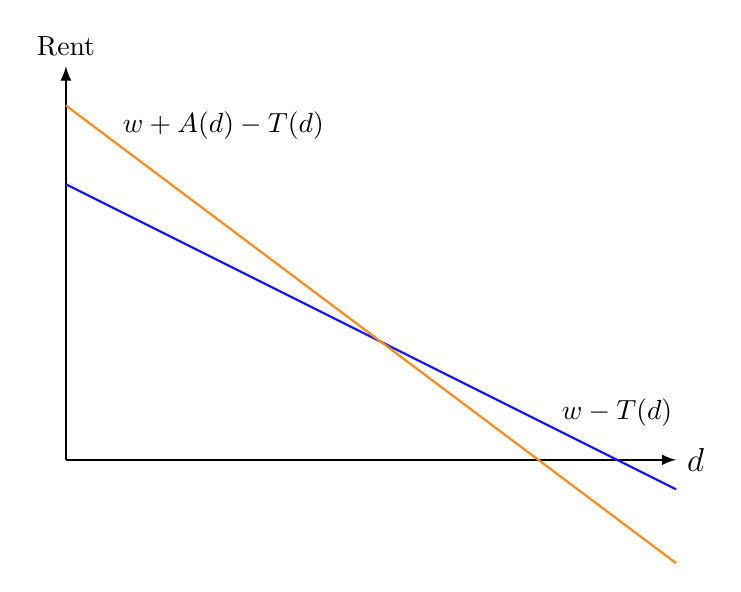
\begin{tikzpicture}[scale=.5]
\def\bndmax{5}        %https://tex.stackexchange.com/questions/68462/filling-a-complex-region-with-tikz
\def\bndmin{0.2}
\def \n {10}
\def \m {15.5}
\def \t {.5}
\def \th {1}
\def \w {7}
\tikzset{func/.style={thick,color=blue!90}}	
\draw [thick, latex-] (0,\n)node[above] {Rent}--(0,0);
\draw [thick, -latex] (0,0)--(\m,0)node[right=.25]{\large $d$};
%\foreach \xi in {0,..., \m} \draw (\xi,0)--(\xi,-.1)node[below=1]{\small$\xi$};
%\foreach \yi in {1,...,\n} \draw (0,\yi)--(-.1,\yi)node[left]{$\yi$};
%%\foreach \i in {1,4,9,16} {
	\draw[func,domain=0:\m] plot [samples=200] (\x,{\w-\t*\x});
%	\draw[func,domain=0:\m, dashed] plot [samples=200] (\x,{\w+\azero-\th*\x+\aprime*\x});

\node at (14,1.2){$w-T(d)$};
\def \azero{2}
\def \aprime {-.25}	
\tikzset{func/.style={thick,color=orange!90}}	
	\draw[func,domain=0:\m] plot [samples=200] (\x,{\w+\azero-\t*\x+\aprime*\x});
\node at (4,8.5){$w +A(d)-T(d)$};
%\node at(-.8,2) [left]{base $2^1=$};
%\node at(-.8,1) [left]{$2^0=$};
%\draw[dotted] (0,2)--(1,2)--(1,0); 
 \end{tikzpicture}
\end{center}
\caption{Rent profile with amenities}
\label{fig-amenity}
\end{figure}

\section{Some simple results}
 This model produces  variations on the standard result in the Alonso model (land rent declining linearly with distance) as the blue line in Figure~\ref{fig-amenity} shows.  If $A(0)>0$, the rent profile is raised near the centre as the  orange line illustrates. Depending on the distance parameter, the city extent may be larger of smaller.  If somehow amenity were to fall below zero in the outer regions of the city as illustrated by the orange line  in Figure~\ref{fig-amenity}, the geographical size of the  city will be smaller. With a linear function this happens if $\frac{a}{b} < \frac{w}{t}$. There would be a band of land around the city with negative amenity for commuters.\footnote{The very simple graphical result rests on several assumptions - no other housing expense, housing all the same size, wages all equal, preferences identical, transportation costs.}

The far more likely case is that $A(d) > 0$ when $w-T(d)$ falls to zero. In this case there is a band of  residents around the city, outside of the population commuting to work. They do not travel to work,  do not collect a wage, but still enjoy the amenity of being close to a city. This might be a population of retired persons enjoying occasional visits and healthcare facilities.

The triangle below the orange line is rent accruing to landowners. \textbf{Total land rent will be higher at the centre of a city with higher amenity}. The  higher rent comes not from desire to be close to the source of the wage income, but from household demand for amenity.  

\section{More complex effects}
Housing choice is always the purchase of  a bundle of characteristics such as location, building space, yard, local density and local amenities. It involves budget allocation. If we hold the housing budget constant and add an explicit urban amenity, other variables must adjust. 

If we hold features of the housing constant,
since employers will not willingly pay for the amenity, some amenities may be financed publicly. It is common to introduce the cost of generating amenities as a tax on residents. Publicly financed amenities, however, may work as a wage subsidy.  
 % \textbf{A city with higher amenity may have a lower equilibrium wage.} (When will this occur?)
   


% \section{Sort}
% {MOVE TO FUTURE WORK/MENTION AMENITY APPENDIX? If the city generates additional social amenities\index{amenities} not captured in the wage  the money available for housing does not change, although willingness to pay must be higher. The most likely adjustments are in urban `subsistence' and it is probably offset by rural amenity that is given up to live in the city. In the long run urban amenities must exert upward pressure on rural amenities.} % These interesting extension will not be taken up in this thesis.}




%Agglomeration amenity is likely to raise wages outside of the city through competition if the overall labour supply is fixed and labour is used outside of the city.



% \section{Rent}
% In Figure~\ref{fig-amenity}, the height of the orange line above $\omega$ represents the rental value of a property at $d$, which is 
% \begin{equation}
% Rent(d)  =  w  + A(d) - T(d)	
% \label{eqn-rent-at-d}\end{equation}
%  and the area under the orange line represents the total rent collected.
%  \footnote{The cost of transportation is a real cost, but the decline in amenity with distance is not.}
 
%  If we solve $w-T(d)=0$ for $d$, we get the maximum  distance workers will commute, $c^{max}$. 
% If we solve $w+A(d)-T(d)=0$ for $d$, we get the maximum  distance at which living near the city offers an advantage, $d^{max}$. For analytical convenience let's assume amenity and transportation are both linear functions of $d$:
% \begin{eqnarray}
% w+ a_0 - b*d^{max} - t*{max}  	&=0		\nonumber \\
% w+a_0 - (b+t)d^{max}  	&=0			\nonumber \\
% d^{max}				&= \frac{w+a_0}{b+t}
% \end{eqnarray}
% For the case of a circular city the area within this radius is $\pi \left(\frac{w+a_0}{b+t}\right)^2$ 




% \subsection{Larson and Yezer quote goes where? if?}
% NOTE: Larson and Yezer \cite{larsonEnergyImplicationsCity2015}  "Virtually all of these applications have involved closed cities with exogenous population, a single type of structure, and exogenous urban transportation costs. None of these efforts has attempted to simulate the effects of variation in city size. The model formulated and solved here is, along with Rappaport (2014), the first urban simulation model of an open city with endogenous population, housing supply and demand, and highway use and congestion. 

}